\chapter{MÔ HÌNH HÓA}
     \section{Mô hình hóa động học xe dò line}
          \hspace*{0.6cm}Trong chương này, nhóm thực hiện mô hình hóa robot, nhằm mục đích hiểu rõ về cấu trúc của xe, phục vụ cho việc thiết kế bộ điều khiển PID bám line cho xe.
          \newline
          \hspace*{0.6cm}Mục đích của điều khiển các động cơ DC để xe di chuyển bám line trên sa bàn trong điều kiện khá lý tưởng, với tải trọng đặt trên xe là cố định, do đó chương mô hình hóa chỉ tập trung vào xây dựng mô hình động học cho xe mà không quan tâm 
          gì đến mô hình động lực học của xe.
          \begin{figure}[H]
               \centering
               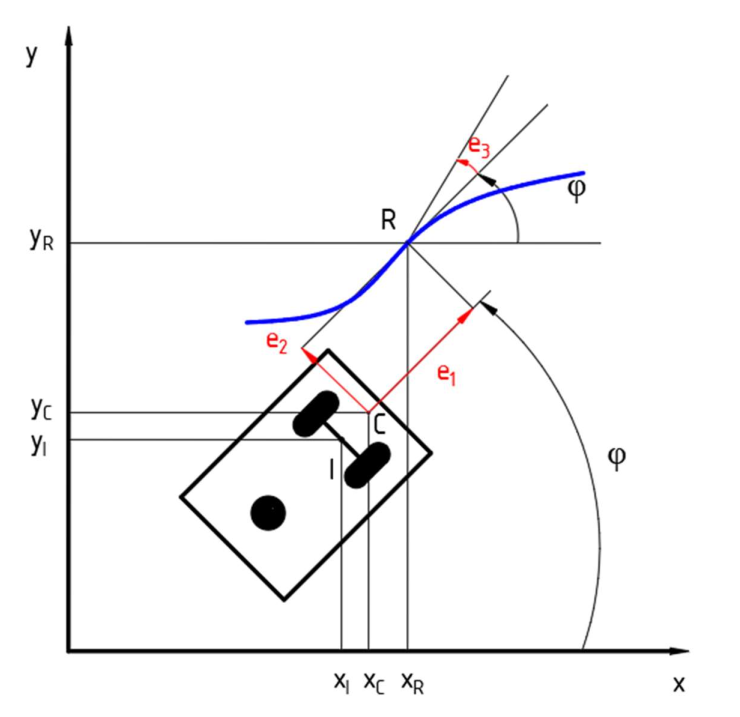
\includegraphics[width=0.7\textwidth]{pictures/chapter5/chapter5_pic1.png}
               \caption{Mô hình động học xe dò line}
               \label{kinematic_model}
          \end{figure}         
          Hình trên mô tả tọa độ các điểm cần thiết của xe trên mặt phẳng tọa độ. Trong đó
          \begin{itemize}
               \item $I(x, y)$: Trung điểm đoạn nối tâm 2 bánh chủ động.
               \item $C(x, y)$: Tâm dãy cảm biến dò line.
               \item $R(x, y)$: Tọa độ điểm tham chiếu trên đường line.
          \end{itemize}
          \hspace*{0.6cm}Phương trình động học tại $I$
          \begin{align*}
               v_{xI} &= \dot{x_I} = v \times \cos \varphi\\
               v_{yI} &= \dot{y_I} = v \times \sin \varphi\\
               \dot{\varphi_I} &= \omega
          \end{align*} 
          Đưa về dạng ma trận
          \begin{align}
               \begin{bmatrix}
                    \dot{x_I} \\
                    \dot{y_I} \\
                    \dot{\varphi_I}
                    \end{bmatrix} &= \begin{bmatrix}
                    \cos\varphi & 0 \\
                    \sin\varphi & 0 \\
                    0 & 1
                    \end{bmatrix} \begin{bmatrix}
                    v \\
                    \omega
               \end{bmatrix}
               \label{c5_e1}
          \end{align}
          \hspace*{0.6cm}Trong đó
          \begin{equation*}
               \begin{cases}
                    v = \dfrac{1}{2}(v_l + v_r) = \dfrac{r\omega_r + r\omega_l}{2} \\[0.5em]
                    \omega = \dfrac{v_r - v_l}{b} = \dfrac{r\omega_r - r\omega_l}{b}
               \end{cases}               
          \end{equation*}
          \begin{itemize}
               \item $v$: vận tốc dài của xe.
               \item $\omega$: vận tốc góc của robot.
               \item $b$: khoảng cách giữa 2 bánh xe.
          \end{itemize}
          \hspace*{0.6cm}Phương trình động học tại điểm bám line $C$
          \begin{equation}
               \begin{cases}
                    x_C = x_I + d \times \cos \varphi \\[0.5em]
                    y_C = y_I + d \times \sin \varphi \\[0.5em]
                    \varphi_C = \varphi_I = \varphi
               \end{cases}   
               \label{c5_e2}            
          \end{equation}
          \hspace*{0.6cm}Lấy đạo hàm ta được 
          \begin{equation}
               \begin{cases}
                    \dot{x_C} = \dot{x_I} - d \times \sin \varphi \dot{\varphi} \\[0.5em]
                    \dot{y_C} = \dot{y_I} + d \times \cos \varphi \dot{\varphi} \\[0.5em]
                    \dot{\varphi_C} = \dot{\varphi_I}
               \end{cases}
               \label{c5_e3}            
          \end{equation}
          \hspace*{0.6cm}Tương tự, mô hình động học tại điểm tham chiếu $R$ trên đường line
          \begin{align}
               \begin{bmatrix}
                    \dot{x_R} \\
                    \dot{y_R} \\
                    \dot{\varphi_R}
                    \end{bmatrix} &= \begin{bmatrix}
                    \cos\varphi_R & 0 \\
                    \sin\varphi_R & 0 \\
                    0 & 1
                    \end{bmatrix} \begin{bmatrix}
                    v_R \\
                    \omega_R
               \end{bmatrix}
               \label{c5_e4}
          \end{align}
          \hspace*{0.6cm}Phương trình biểu diễn sự sai lệch giữa điểm bám line $C$ và vị trí điểm tham chiếu $R$ mong muốn trên đường line
          \begin{equation}
               \begin{cases}
                    x_R - x_C = e_1 \cos \varphi - e_2 \sin \varphi \\[0.5em]
                    y_R - y_C = e_1 \sin \varphi + e_2 \cos \varphi \\[0.5em]
                    \varphi_R - \varphi_C = e_3
               \end{cases}    
               \label{c5_e5}           
          \end{equation}
          \hspace*{0.6cm}Trong đó
          \begin{itemize}
               \item $e_1$: sai số vị trí giữa điểm bám line $C$ và điểm tham chiếu $R$ theo phương vuông góc với trục hai bánh dẫn động.
               \item $e_2$: sai số vị trí giữa điểm bám line $C$ và điểm tham chiếu $R$ theo phương song song với trục hai bánh dẫn động.
               \item $e_3$: sai số góc giữa hướng của xe và hướng tiếp tuyến với sa bàn tại điểm tham chiếu $R$.
          \end{itemize}    
          \hspace*{0.6cm}Từ phương trình (\ref{c5_e5}) rút ra được hệ phương trình các sai số
          \begin{align}
               \begin{bmatrix}
                    e_1 \\
                    e_2 \\
                    e_3
                    \end{bmatrix} &= \begin{bmatrix}
                    \cos\varphi & \sin \varphi & 0 \\
                    -\sin\varphi & \cos \varphi & 0 \\
                    0 & 0 & 1
                    \end{bmatrix} \begin{bmatrix}
                    x_R - x_C \\
                    y_R - y_C \\
                    \varphi_R - \varphi_C
               \end{bmatrix}
               \label{c5_e6}
          \end{align}
          \hspace*{0.6cm}Đạo hàm 2 vế hệ (\ref{c5_e6}), khai triển và rút gọn ta thu được 
          \begin{align}
               \begin{bmatrix}
                    \dot{e_1} \\
                    \dot{e_2} \\
                    \dot{e_3}
                    \end{bmatrix} &= \begin{bmatrix}
                    v_R \cos e_3 \\
                    v_R \sin e_3 \\
                    \omega_R
                    \end{bmatrix} + \begin{bmatrix}
                    -1 & e_2 \\
                    0 & -d - e_1 \\
                    0 & -1
                    \end{bmatrix} \begin{bmatrix}
                    v_I \\
                    \omega_I
               \end{bmatrix}
               \label{c5_e7}
          \end{align}       
     \section{Tính toán thời gian lấy mẫu}
          \subsection{Tính toán thời gian lấy mẫu cho bộ điều khiển động cơ}
               \hspace*{0.6cm}Nhóm cần tính toán thời gian lấy mẫu cho động cơ \textit{JGB37-520 333RPM} có gắn encoder với các thông số như số vòng quay sau 
               hộp giảm tốc là 333 vòng/phút, 2 kênh encoder với mỗi kênh nhận 11 xung/vòng.\\
               Số vòng quay tối đa của động cơ
               \begin{equation*}
                    333 \,\mathrm{rpm} = \dfrac{333}{60} \,\mathrm{rev/s} = 5.55 \,\mathrm{rev/s}
               \end{equation*}
               Sử dụng 2 kênh encoder với chế độ quadrature, nghĩa là mỗi vòng encoder đếm tổng cộng $11 \times 4 = 44 \,\mathrm{xung}$.\\
               Tần số xung và thời gian giữa 2 lần đếm xung của encoder là 
               \begin{align*}
                    &f_{\text{pulse}} = 44 \times 5.55 = 244.2 \,\mathrm{Hz}\\
                    &T_{\text{pulse}} = \dfrac{1}{244.2} = 4.095 \,\mathrm{ms}
               \end{align*}
               Sử dụng tiêu chuẩn Nyquist, tần số tối thiểu (tương đương với thời gian lấy mẫu tối da để khôi phục tín hiệu xung) là 
               \begin{align*}
                    &f_s \geq 2 f_{\text{pulse}} = 2 \time 244.2 = 488.4 \,\mathrm{Hz}\\
                    &t_s \leq \dfrac{1}{f_s} = \dfrac{1}{488.4} = 2.05 \,\mathrm{ms}
               \end{align*}
               Nếu lấy mẫu theo tiêu chuẩn Nyquist, số lượng xung ở mỗi lần lấy mẫu không đủ, nhiều mẫu bị mất xung, nhóm sử dụng chế độ Encoder Mode của STM32 để tính toán
               số xung encoder trong mỗi lần ngắt để tính toán tốc độ động cơ làm giá trị phản hồi cho vòng điều khiển, do đó cần lựa chọn khoảng thời gian lấy mẫu sao cho số xung đọc được 
               ổn định để tính toán giá trị vận tốc động cơ. Số xung mà vi điều khiển đọc được trong khoảng thời gian lấy mẫu $t_s$ là 
               \begin{equation*}
                    n = \dfrac{t_s}{T_{\text{pulse}}} = \dfrac{t_s}{4.095}
               \end{equation*}
               Nhóm lựa chọn thời gian lấy mẫu cho bộ điều khiển tốc độ động cơ là $t_s = 0.01 \,\mathrm{s}$.
          \subsection{Tính toán thời gian lấy mẫu cho bộ điều khiển bám line}
               \hspace*{0.6cm}Để tính toán thời gian lấy mẫu cho bộ điều khiển bám line, ta tính toán quãng đường tối đa mà xe di chuyển trên đoạn đường cong 
               có bán kính lớn nhất trong khoảng thời gian giữa 2 lần lấy mẫu mà vẫn đảm bảo được sai số bám line.\\
               \hspace*{0.6cm}Giả sử tâm cảm biến dò line nằm ngay tại vị trí tâm đường line tại thời điểm đầu, tại thời điểm lấy mẫu kế tiếp, với mong muốn sai số $e_2$ giữa tâm đường cảm biến 
               và tâm line không lệch nhau quá 3mm. Do đó quãng đường AB lớn nhất mà xe chạy được trước khi đạt tới sai số 3mm là 
               \begin{equation*}
                    AB = \sqrt{OB^2 - OA^2} = \sqrt{(OA + e_{2max})^2 - OA^2}
               \end{equation*}
               Trong đó 
               \begin{itemize}
                    \item $OA$ là bán kính của đường cong.
                    \item $e_{2max}$ là khoảng sai số lớn nhất khi di chuyển trên cung.
               \end{itemize}
               Ta thấy khi $OA$ càng lớn thì khoảng di chuyển trên cung của xe càng lớn, ta tính toán với bán kính $OA = 800 \,\mathrm{mm}$
               \begin{equation*}
                    AB = 69.34 \,\mathrm{mm}
               \end{equation*}
               Để xe có thể bám được line khi vào đoạn đường cong trên thì thời gian lấy mẫu cho bộ điều khiển vị trí bám line phải thỏa
               \begin{equation*}
                    t_{\text{đk}} \leq \dfrac{AB}{v} = \dfrac{69.34}{300} = 0.23 \,\mathrm{s}
               \end{equation*}
               $v$ là vận tốc của xe khi vào cua: $v = 300 \,\mathrm{mm/s}$.
               Ta chọn $t_{\text{đk}} = 0.05 \,\mathrm{s}$.

     \section{Mô hình hóa động cơ}
          \hspace*{0.6cm}Thực hiện mô hình hóa động cơ, tìm hàm truyền động cơ bằng cách xem xét mối quan hệ giữa đầu vào giá xung PWM và đầu ra là tốc độ quay của trục động cơ (vòng/phút).   
          \subsection{Mô hình hóa động cơ dẫn động bánh phải}    
               \hspace*{0.6cm}Sử dụng driver TB6612FNG, sau khi cấp xung và đo tốc độ động cơ, thu được bảng số liệu sau
               \begin{table}[h!]
                    \centering
                    \begin{tabular}{|c|c|}
                         \hline
                         \textbf{\%PWM} & \textbf{RPM} \\
                         \hline
                         0 & 0 \\
                         5 & 0 \\
                         10 & 0 \\
                         15 & 9.0909 \\
                         20 & 22.7273 \\
                         25 & 45.4545 \\
                         30 & 63.6364 \\
                         35 & 77.2727 \\
                         40 & 95.4545 \\
                         45 & 109.0909 \\
                         50 & 122.7273 \\
                         55 & 131.8182 \\
                         60 & 154.5455 \\
                         65 & 172.7273 \\
                         70 & 181.8182 \\
                         75 & 195.4545 \\
                         80 & 209.0909 \\
                         85 & 227.2727 \\
                         90 & 236.3636 \\
                         95 & 254.5454 \\
                         100 & 263.6364 \\
                         95 & 268.1818 \\
                         90 & 263.6364 \\
                         85 & 250.0000 \\
                         80 & 240.9091 \\
                         75 & 231.8182 \\
                         70 & 218.1818 \\
                         65 & 204.5455 \\
                         60 & 186.3636 \\
                         55 & 177.2727 \\
                         50 & 154.5455 \\
                         45 & 140.9091 \\
                         40 & 136.3636 \\
                         35 & 127.2727 \\
                         30 & 100.0000 \\
                         25 & 86.3636 \\
                         20 & 63.6364 \\
                         15 & 45.4545 \\
                         10 & 36.3636 \\
                         5 & 22.7273 \\
                         0 & 0 \\
                         \hline
                    \end{tabular}
                    \caption{Quan hệ giữa \%PWM và tốc độ quay (RPM)}
               \end{table}
               \newpage
               \hspace*{0.6cm}Đáp ứng của động cơ bánh phải theo thời gian
               \begin{figure}[H]
                    \centering
                    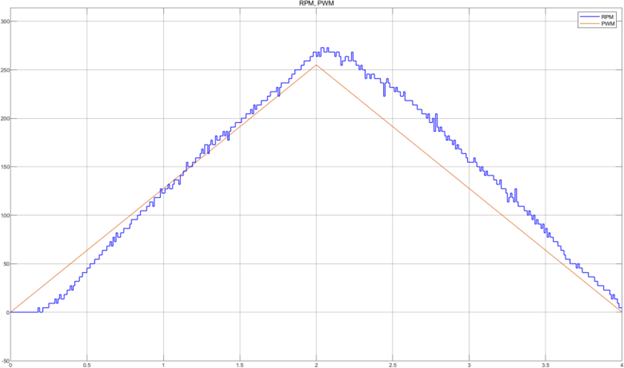
\includegraphics[width=1\textwidth]{pictures/chapter5/CJGB1_response.png}
                    \caption{Đáp ứng của động cơ bánh phải}
                    \label{CJGB1_response}
               \end{figure}  
               \hspace*{0.6cm}Sử dụng Toolbox System Identification của Matlab ta có hàm truyền của động cơ bánh phải 
               \begin{figure}[H]
                    \centering
                    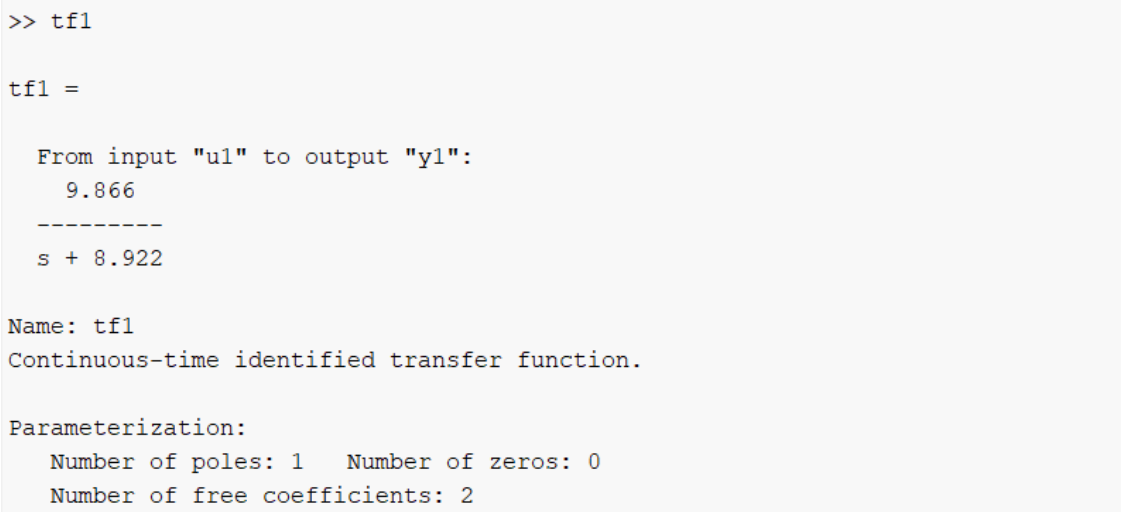
\includegraphics[width=1\textwidth]{pictures/chapter5/CJGB1_tf.png}
                    \caption{Hàm truyền động cơ bánh phải}
                    \label{CJGB1_tf}
               \end{figure} 
               \hspace*{0.6cm}So sánh giữa đáp ứng thực tế và hàm truyền của động cơ bánh phải
               \begin{figure}[H]
                    \centering
                    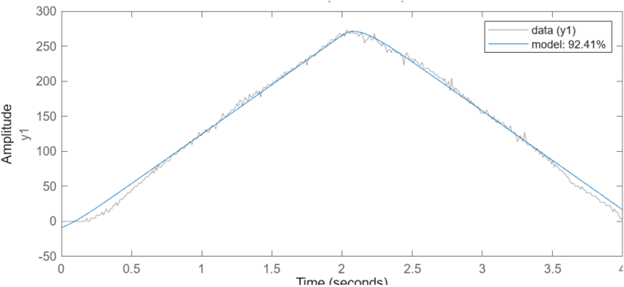
\includegraphics[width=1\textwidth]{pictures/chapter5/CJGB1_compare.png}
                    \caption{Hàm truyền động cơ bánh phải}
                    \label{CJGB1_compare}
               \end{figure} 
          \subsection{Mô hình hóa động cơ dẫn động bánh trái}
               \hspace*{0.6cm}Tương tự như thu thập dữ liệu bánh phải động cơ, sau khi cấp xung và đo tốc độ động cơ, thu được bảng số liệu sau
               \begin{table}[h!]
                    \centering
                    \begin{tabular}{|c|c|}
                         \hline
                         \textbf{\%PWM} & \textbf{RPM} \\
                         \hline
                         0   & 0 \\
                         5   & 4.55 \\
                         10  & 0 \\
                         15  & 18.18 \\
                         20  & 31.82 \\
                         25  & 50.00 \\
                         30  & 59.09 \\
                         35  & 63.64 \\
                         40  & 100.00 \\
                         45  & 122.73 \\
                         50  & 145.45 \\
                         55  & 145.45 \\
                         60  & 159.09 \\
                         65  & 163.64 \\
                         70  & 186.36 \\
                         75  & 200.00 \\
                         80  & 218.18 \\
                         85  & 231.82 \\
                         90  & 245.45 \\
                         95  & 272.73 \\
                         100 & 277.27 \\
                         95  & 281.82 \\
                         90  & 259.09 \\
                         85  & 268.18 \\
                         80  & 245.45 \\
                         75  & 240.91 \\
                         70  & 222.73 \\
                         65  & 204.55 \\
                         60  & 190.91 \\
                         55  & 181.82 \\
                         50  & 150.00 \\
                         45  & 150.00 \\
                         40  & 122.73 \\
                         35  & 109.09 \\
                         30  & 100.00 \\
                         25  & 90.91 \\
                         20  & 63.64 \\
                         15  & 45.45 \\
                         10  & 31.82 \\
                         5   & 27.27 \\
                         0   & 9.09 \\
                         \hline
                    \end{tabular}
                    \caption{Quan hệ giữa \%PWM và tốc độ quay (RPM)}
               \end{table}
               \newpage
               \hspace*{0.6cm}Đáp ứng của động cơ bánh trái theo thời gian
               \begin{figure}[H]
                    \centering
                    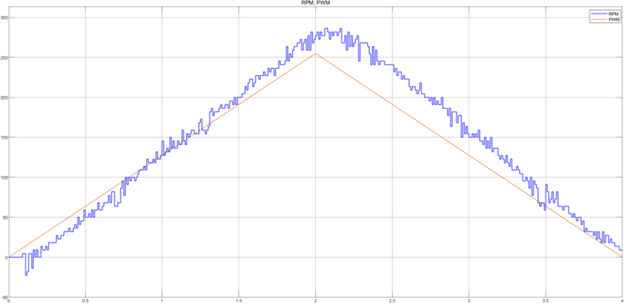
\includegraphics[width=1\textwidth]{pictures/chapter5/CJGB2_response.png}
                    \caption{Đáp ứng của động cơ bánh trái}
                    \label{CJGB2_response}
               \end{figure}  
               \hspace*{0.6cm}Sử dụng Toolbox System Identification của Matlab ta có hàm truyền của động cơ bánh trái 
               \begin{figure}[H]
                    \centering
                    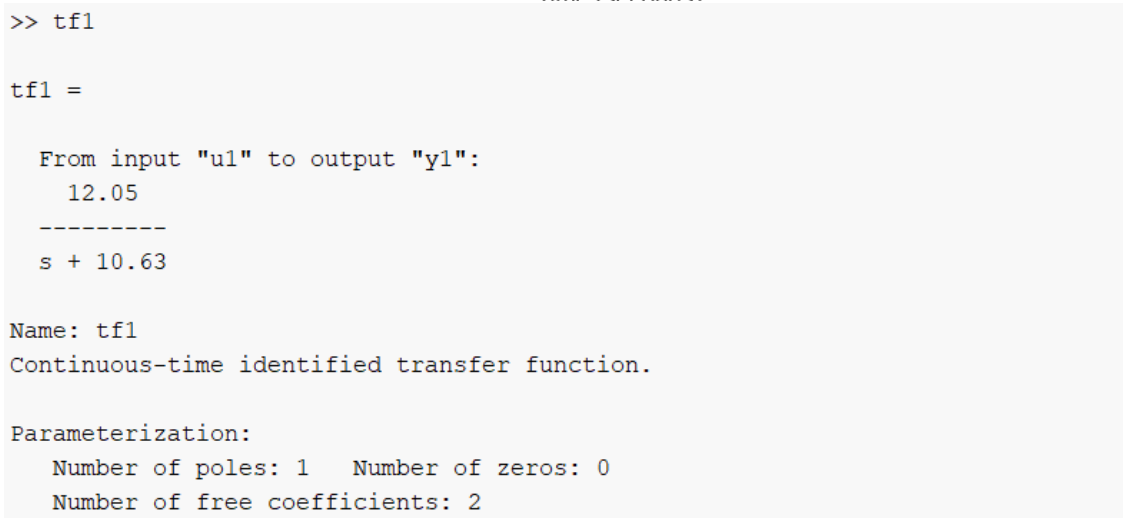
\includegraphics[width=1\textwidth]{pictures/chapter5/CJGB2_tf.png}
                    \caption{Hàm truyền động cơ bánh trái}
                    \label{CJGB2_tf}
               \end{figure} 
               \hspace*{0.6cm}So sánh giữa đáp ứng thực tế và hàm truyền của động cơ bánh trái
               \begin{figure}[H]
                    \centering
                    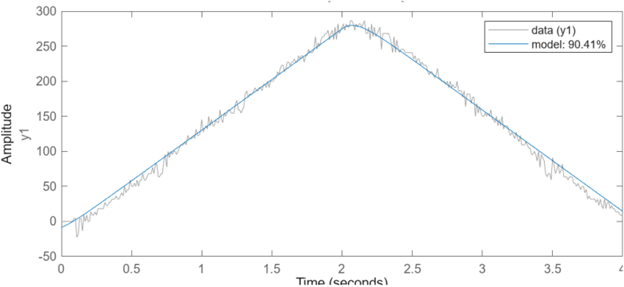
\includegraphics[width=1\textwidth]{pictures/chapter5/CJGB2_compare.png}
                    \caption{Hàm truyền động cơ bánh trái}
                    \label{CJGB2_compare}
               \end{figure}
     




          


